\subsection{Architecture}
To create and manage independent processing infrastructure we used Docker containers. This enables the application to run on different machines with different operating systems having Docker and Compose installed as the only requirement. 

The containers are started by Docker Compose. There is a driver container that launches Jupyter notebooks on \url{http://localhost:8888} and can run python notebooks with pynb. 
Jupyter notebook is an open-source tool for data science, that allows the users to execute scripts in an interactive fashion. It supports different programming languages and frameworks such as Python, R, pySpark and so on. It is mostly used for prototyping, since it is not suitable for clean and sustainable code with proper version control. Also it is not possible to automate running Jupyter notebooks as tasks. 
Pynb is a tool that allows to convert Jupyter notebooks to plain python code and vice verse. The maintenance of such python notebooks is more sustainable and it is possible to programatically run them. \cite{pynb}

The driver runs pySpark applications on the baseline standalone Spark\footnote{Spark is a data analytics engine for big data processing, with built-in modules for streaming, SQL, machine learning and graph processing. For more details refer to \cite{spark}.} cluster with one worker and one master with client deploy mode. In standalone cluster mode, Spark's own cluster manager is used instead of YARN or Mesos. Client deploy mode means that  the driver is launched in the same process as the client that submits the application. 

A master container that deploys Spark master, and a worker container that starts a worker with one core and 1 gigabyte of memory, connected to the master. The Spark web user interface shows the available worker on \url{http://localhost:8080}.

As a data-source we prefer Parquet\footnote{Apache Parquet is a columnar storage format designed for the Hadoop ecosystem, independent of the data processing framework, data model or programming language. For more details see \cite{parquet}.} over .csv, since most of the operations in the project involve iterating through all rows for given columns. This way we take advantage of the Parquet being an efficient columnar storage.

The project is written in Python 3 and it heavily utilizes the DataFrame API within Spark SQL. A DataFrame in pySpark is an immutable distributed collection of data. However, in contrast with an RDD, data is organized into named columns, akin to a table in a relational database, designed to make large data sets processing very easy.

We use Fabric to orchestrate the containers, run tests and execute tasks. It is more convenient to use a unified command line interface for recurring administration tasks. \cite{fabric}

\subsection{Data sets}
The following data sources are used:
\begin{itemize}
\item Cell map Data: OpenCelliD public data set representing cell tower locations and meta data.
\item CDR data: Sequences of network connections together with actual GPS location (recording every second the information about neighbouring cell towers including the connected one)
\end{itemize}

\subsubsection{Cell map data set}
The full data set of OpenCelliD was downloaded as of 14 April 2018 from \url{https://opencellid.org/downloads.php}. The downloaded .csv file is 3.1 GB on disk. The following attributes of OpenCelliD data set are used for the analysis \cite{opencellid}:
\begin{itemize}
\item radio: \textit{string} - Network type. One of the strings GSM, UMTS, LTE or CDMA.
\item mcc:  \textit{integer}  -  Mobile Country Code, for example 262 for Germany.
\item net: \textit{integer} - For GSM, UMTS and LTE networks, this is the Mobile Network Code (MNC). For CDMA networks, this is the System Identification number (SID).
\item cell: \textit{integer} - Cell ID (CID) for GSM and LTE networks. UTRAN Cell ID / LCID for UMTS networks, which is the concatenation of 2 or 4 bytes of Radio Network Controller (RNC) code and 4 bytes of Cell ID. Base station identifier number (BID) for CDMA networks.
\item lat: \textit{double} - Latitude in degrees between -90.0 and 90.0.
\item lon: \textit{double} - Longitude in degrees between -180.0 and 180.0.
\item samples: \textit{integer} - Total number of measurements assigned to the cell tower.
\item changeable:  \textit{integer} - Defines if coordinates of the cell tower are exact or approximate. \footnote{changeable=1: the GPS position of the cell tower has been calculated from all available measurements. changeable=0: the GPS position of the cell tower is precise - no measurements have been used to calculate it.}
\item created: \textit{integer} - The first time when the cell tower was seen and added to the OpenCelliD database. \footnote{A date in time stamp format: number of seconds since the UTC Unix Epoch of 1970-01-01T00:00:00Z (For example 1409522613 is the time stamp for 2014-08-31T22:03:33Z).}
\item updated: \textit{integer} - The last time when the cell tower was seen and updated.
\end{itemize}

We expect less cell towers in the outskirts of the city and more towards the center. Figure \ref{fig:opencellid}\footnote{Only the latest observations are shown.} shows that the density of cell towers within Telfonica network from OpenCelliD is quite dense even in the outer regions of Berlin. Thus the data from OpenCelliD might be corrupted or of poor quality.

\begin{figure}[h]
    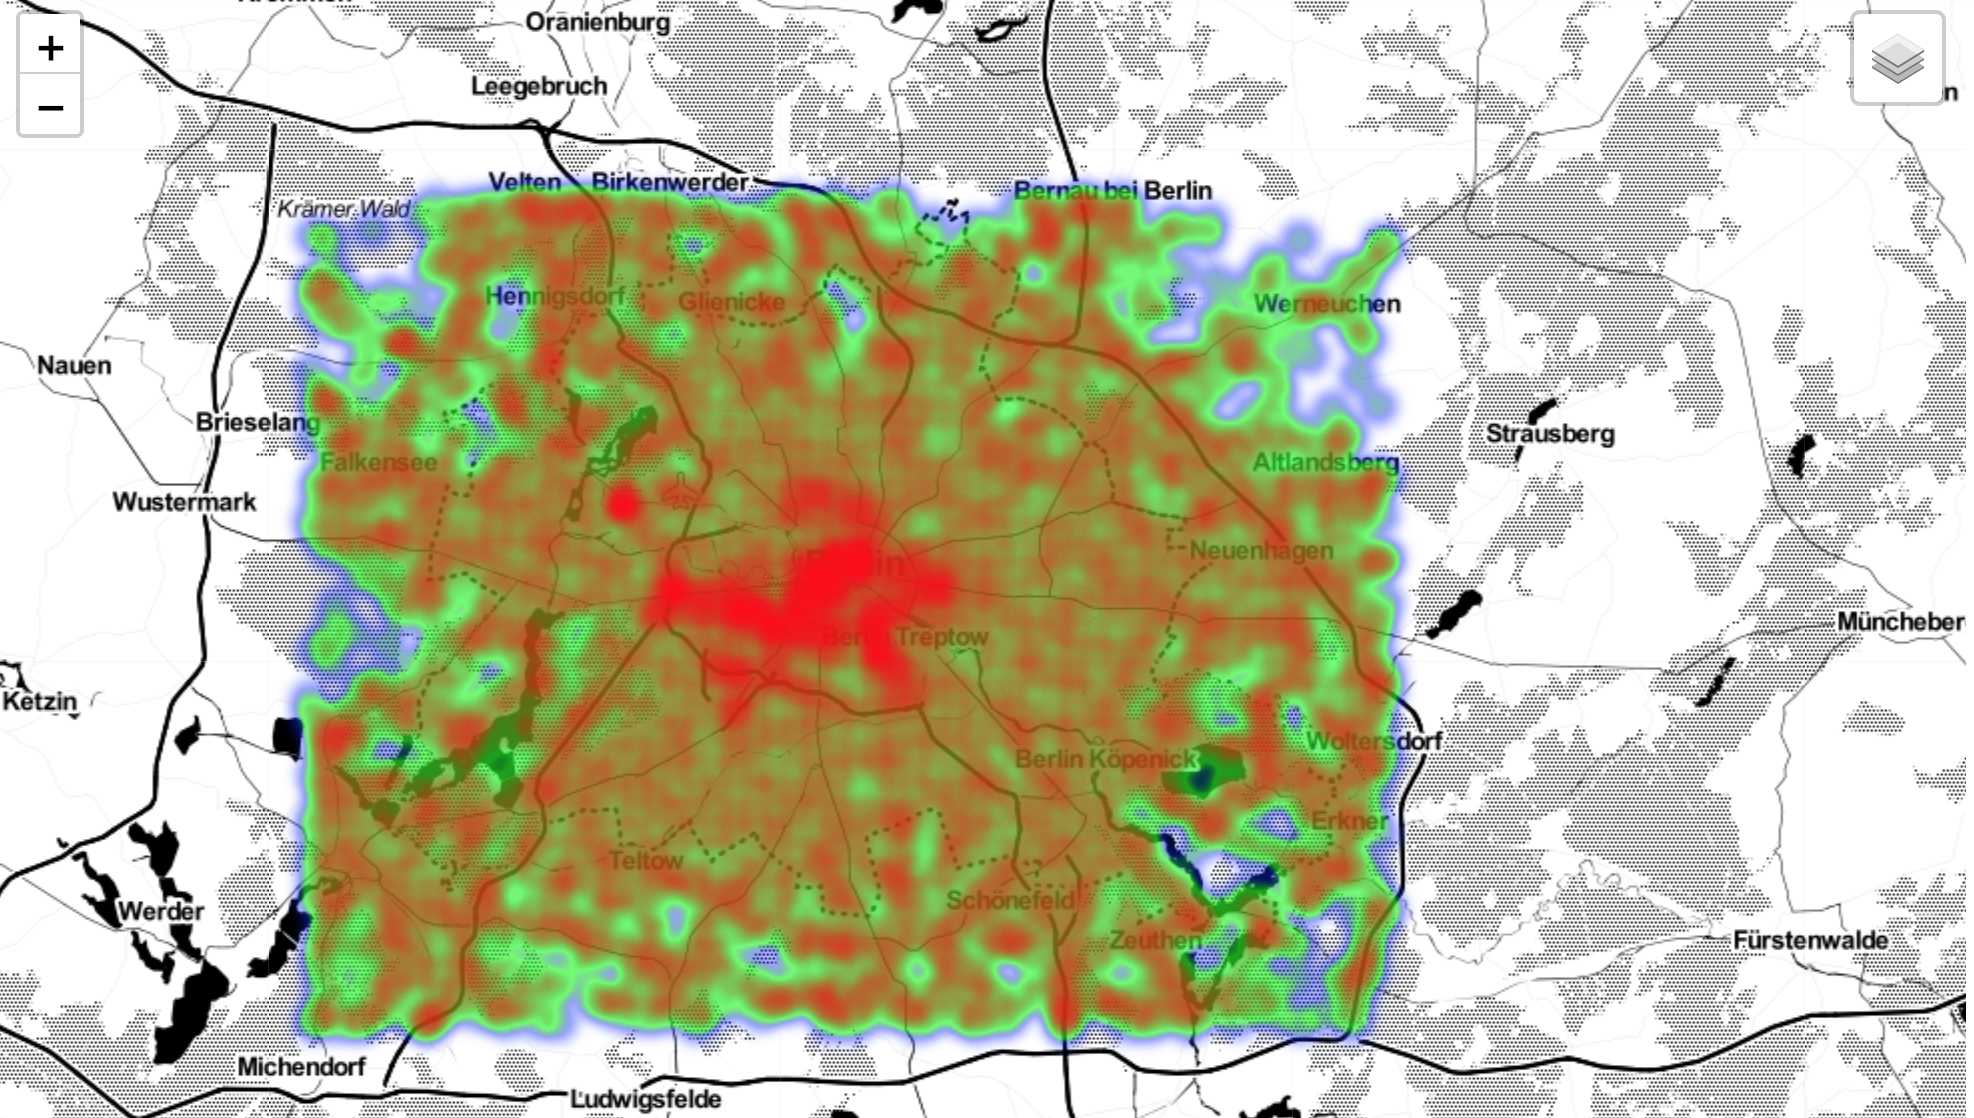
\includegraphics[width=0.5\textwidth]{images/opencellid.png}
    \caption{Heat map of Telefonica cell towers in Berlin (Source: OpenCelliD) }
    \label{fig:opencellid}
\end{figure}

\subsubsection{CDR data}
The CDR data set was generated between 2018-03-12 and 2018-03-16 in Berlin region with a custom application illustrated in Figure\ref{fig:app} using Nexus 4 E960 test phone (Android operating system). The CDR data includes features such as:
\begin{itemize}
\item system\_time: \textit{integer} - Date and time when event was generated in timestamp format, i.e. the number of seconds since Jan 01 1970. (UTC)
\item unix\_dt: \textit{datetime} - Date and time when event was generated.
\item net: \textit{string} - Type of the network (e.g. GSM, LTE or UMTS).
\item lac: \textit{integer} - Location Area Code of the cell.
\item cisac: \textit{integer} - Cell id.
\item latitude: \textit{double} - Latitude of actual GPS location of the phone.
\item longitude: \textit{double} - Longitude of actual GPS location of the phone.
\end{itemize}

\begin{figure}[h]
    \begin{center}
    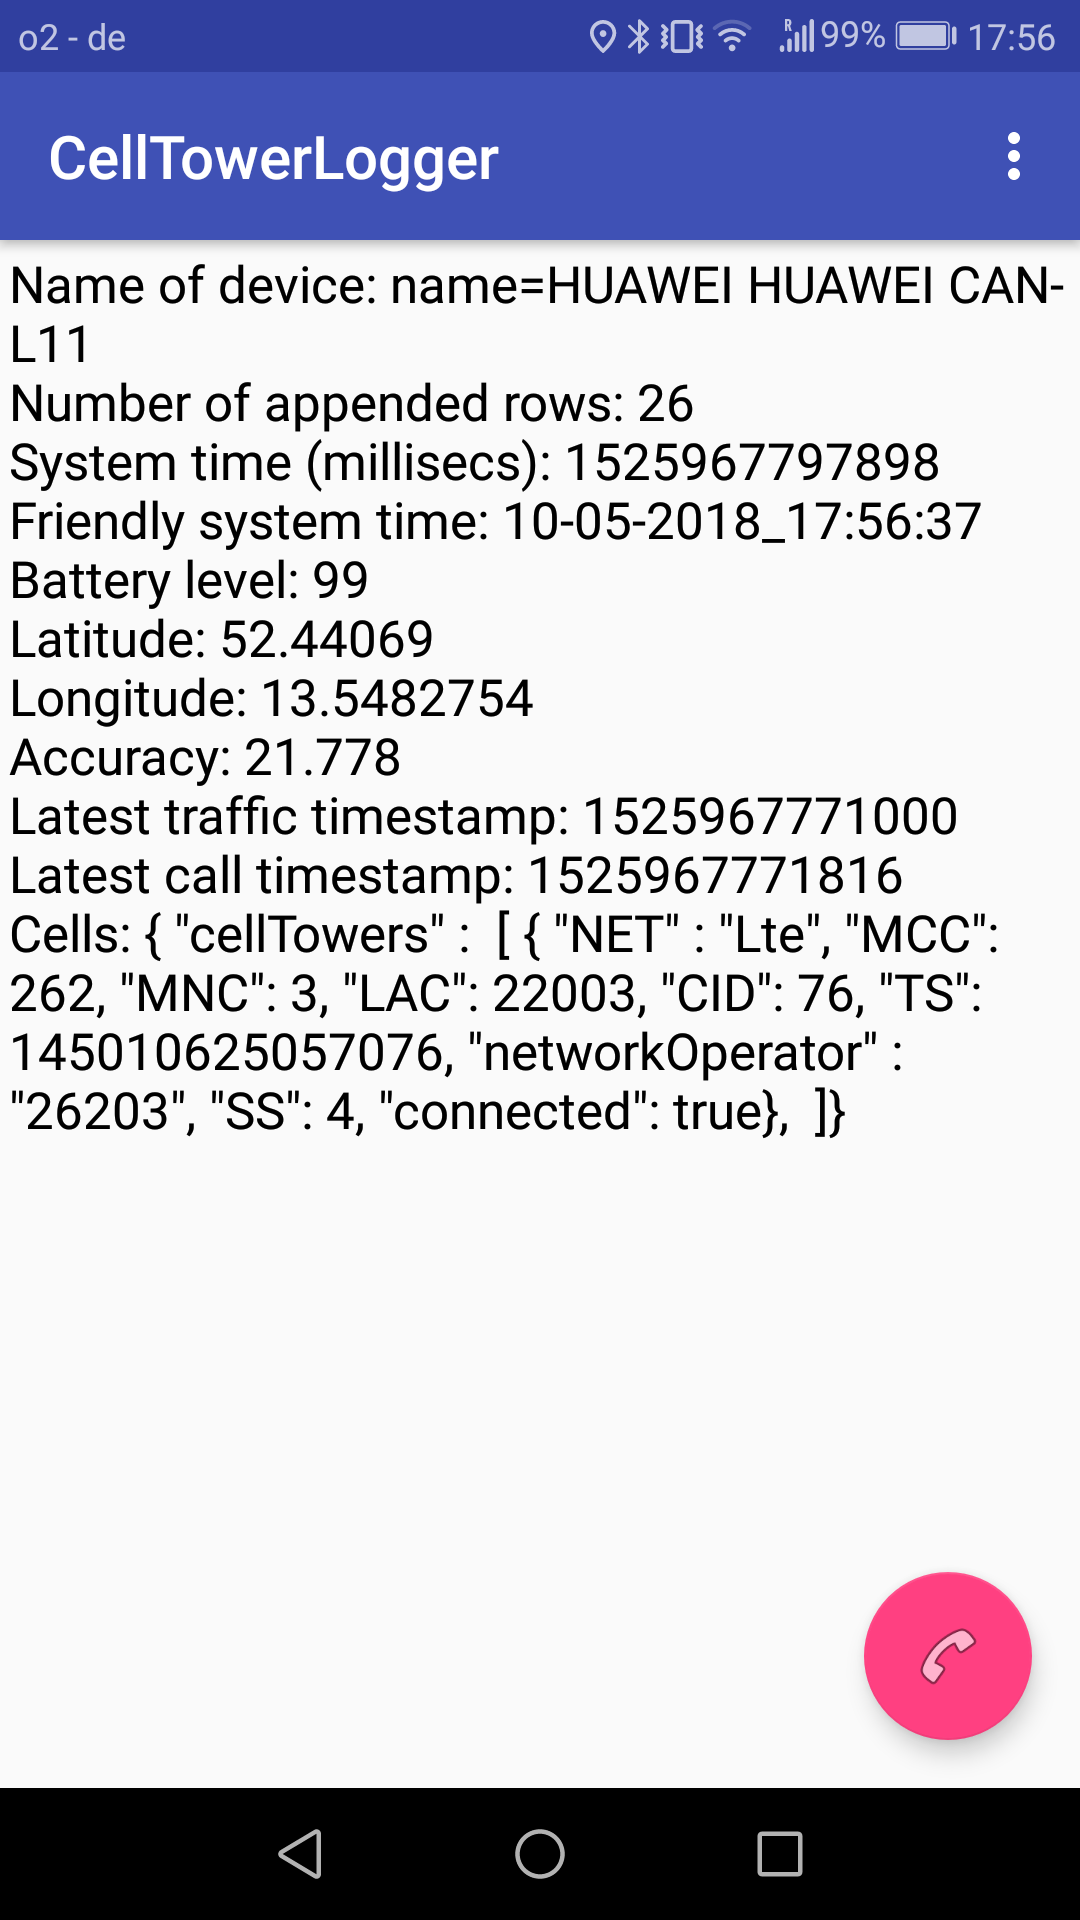
\includegraphics[height=10cm]{images/celltower_logger.png}
    \caption{Android application built for data collection}
    \label{fig:app}
    \end{center}
\end{figure}

There are cell towers that were assigned to the collected events more frequently than others. These are likely to be around the home or workplace of the user generating the data.

On average there was a CDR record logged in about every second during the data collection. However that would be less frequent with real life usage, depending on individual mobile usage preferences. 

By collecting observation in every second, we discretize time and make sure that the trajectories we compare using Euclidean distance have the same number of data points.

\subsection{Data processing}\label{sec:data-proc}
The data-flow throughout the implementation steps can be seen on Figure \ref{fig:data-flow}.
\begin{figure}[h]
    \centering
    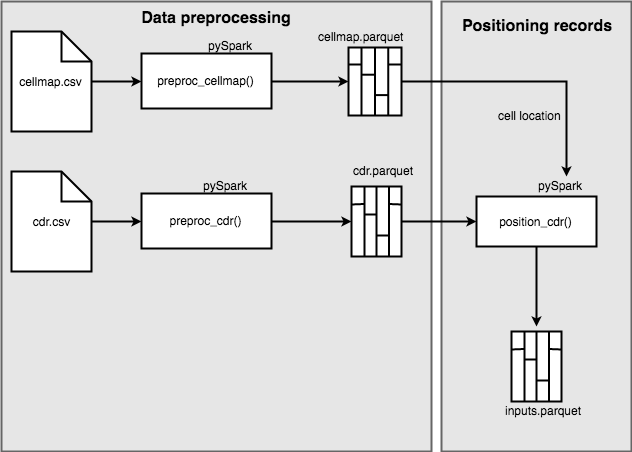
\includegraphics[width=0.5\textwidth]{images/data-flow.png}
    \caption{Data flow}
    \label{fig:data-flow}
\end{figure}

\subsubsection{Data pre-processing}
The cell map files cannot be fit into memory, therefore pySpark is used for the cleaning process with the following steps: 
\begin{enumerate}
    \item Import csv to pySpark DataFrame
    \item Drop irrelevant columns
    \item Keep only the records of cells in the Telefonica network in Berlin
    \item Write cleaned data to parquet files
\end{enumerate}

The CDR data-set generated by the test phone in the given time period is stored in a single .csv file. The size of real-world mobile network events generated daily can go up to hundreds of gigabytes per day. The following steps are executed during the pre-processing: 
\begin{enumerate}
   \item Import .csv files to pySpark DataFrame
    \item Clean data:
    \begin{itemize}
        \item Fetch data from JSON column to data frame columns
        \item Create cell(lac, cisac) column
        \item Convert unix timestamp to datetime with Central European Timezone (CET)
    \end{itemize}
    \item Write data to Parquet files
\end{enumerate}

The DataFrames are re-partitioned before writing them to Parquet files to avoid having a large number of tiny files for a relatively small data. 

\subsubsection{Positioning mobile network events}
Having preprocessed the raw data, the next step is to assign a location to each of the events in the CDR data-set from the cell map data-set based on the respective cell tower id. 
These steps are executed for positioning the CDR data:
\begin{itemize}
    \item Load CDR data from parquet files to pySpark DataFrame
    \item Load cell map data to pySpark DataFrame
    \item Prepare imported DataFrames
    \item Join CDR and cell map data-sets on cell id
    \item Calculate Haversine distances
    \item Keep rows with distance less than 10 kilometers
    \item For each event keep only the closest cell tower\footnote{In the OpenCelliD data set there are several observations with the same cell ID and we only want to keep the one that is closest to the GPS location of the events.}
    \item Persist joined DataFrame to parquet files
\end{itemize}
